\chapter{The bot}
	\section{The architecture}
	The architecture of the bot is divided in four categories:
	\begin{figure}[H]
		\centering
		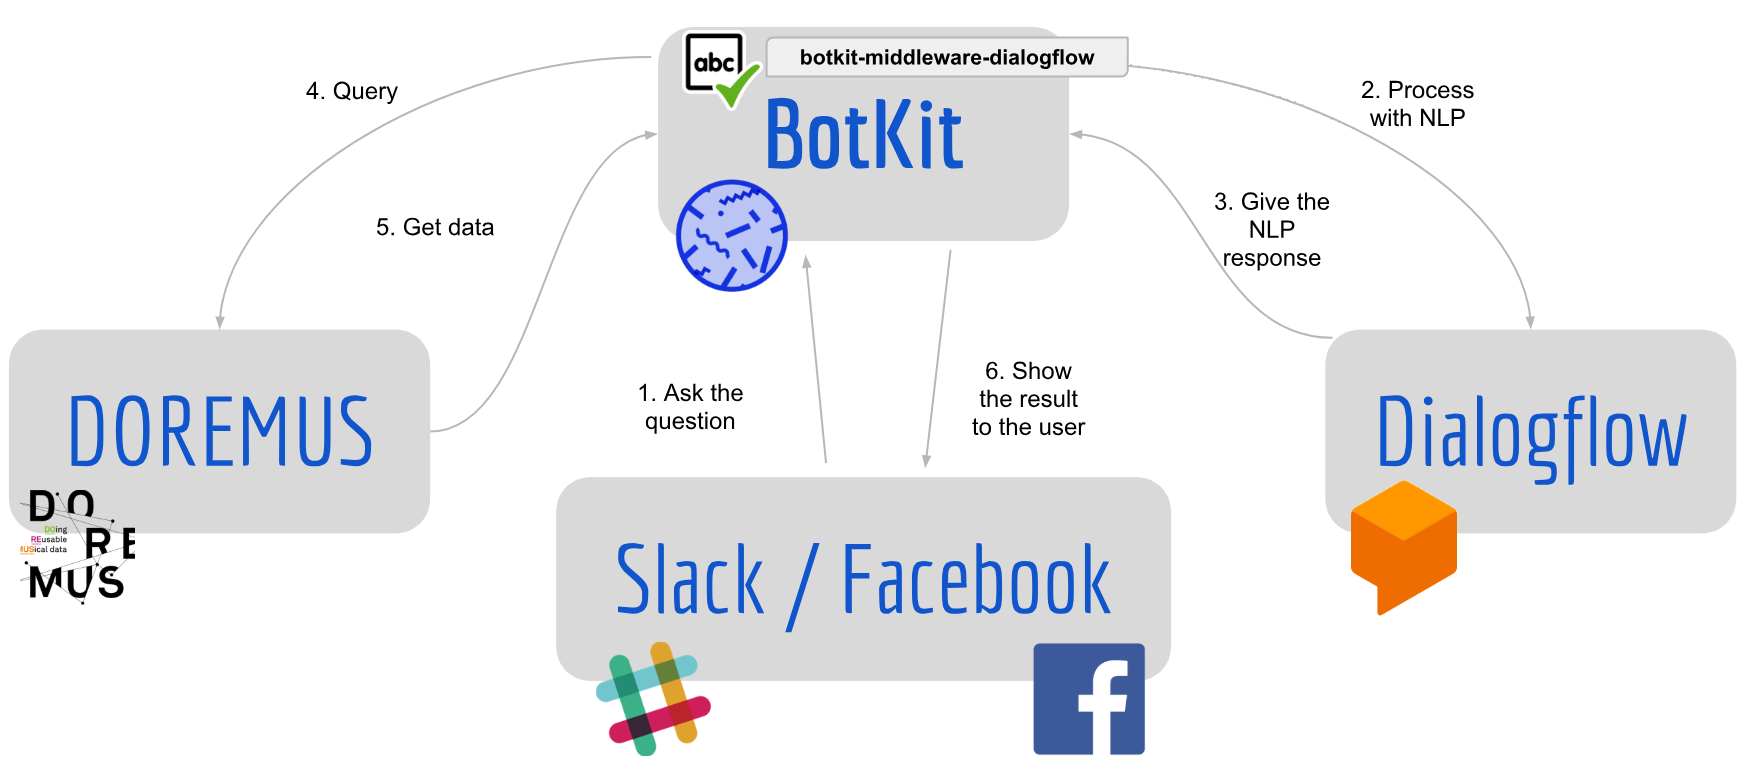
\includegraphics[scale=0.2]{arch2}
		\caption{The high-level architecture of DOREMUS Bot.}
	\end{figure}
	First of all we can find the client, that in the case of our development, testing and validation process, has been \textit{Slack}. Of course, it can be any of the clients which support the installation of the bot on it (\textit{Telegram}, \textit{Facebook Messenger}, etc.). The use of Slack let us to exploit the beautiful \textit{Slack Cards}, to make the answers of our bot (works, artists, performances) prettier and easier to understand at a glance. A set of examples will be provided in the last chapter.\\\\
	The second part of the architecture is represented by the NLP. In this case, as told in the previous chapter, we used \textit{Dialogflow}, to exploit its advanced slot-filling techniques and its NLU power.\\\\
	However, we didn't use \textit{Dialogflow} on its own, exploiting the direct integration with \textit{Slack}, but we used something that we placed in the middle of the two: \textit{Botkit}. \textit{Botkit} is a bot-making toolkit that aims to ease the building process of a bot, potentially exploiting different NLPs and/or different clients. In our case, \textit{Botkit} has been deployed on a web server, and thanks to the \textit{NodeJS} code we were able to come up with a series of features (like the spell checker) that would have been impossible to reach with a simple (direct) integration between \textit{Slack} and \textit{Dialogflow}. We'll talk more about that in the following paragraphs. The communication with the \textit{Dialogflow} NLP is done thanks to a modified version of the \texttt{botkit-middleware-dialogflow}\cite{bmd}: there will be a paragraph dedicated to this middleware in the following pages.\\\\
	The last part of the architecture is of course represented by the data source: \textit{DOREMUS}. We talked about that in the previous chapters, but from the architecture is important to notice how the knowledge graph is queried: each query is dynamic, in the sense that according to the intent, the number of filters and the desired results wanted by the user, the query will have a different shape and a different content. The bot code is able to add different pieces of queries according to what \textit{Dialogflow} is able to understand and to provide as output values of the API.\\\\
	The bot code is organized in this way:
	\begin{lstlisting}
	
	bot.js
	spell-checker-middleware.js
	logger.js
	
	config/
		.env
	
	doremus/
		bot_functions.js
	
	slack/
		slack_io.js
		slack_cards.js
	
	facebook/
		facebook_io.js
		facebook_cards.js
		
	dialogflow/
		index.js
		functions.js
		io.js
	\end{lstlisting}
	where:
	\begin{itemize}
		\item \texttt{bot.js} is the entry point of the node application. It contains the code to declare the fundamental libraries, to start the RTM, and to load the hears methods.
		
		\item \texttt{spell-checker-middleware.js} is the custom module to perform the spell-checking before sending the received sentences to the NLP.
		
		\item \texttt{logger.js} is the module which logs various informations inside the log files (created in the \texttt{log\_folder} specified in the \texttt{.env} file).
		
		\item \texttt{.env} is the secret file (to place into the \texttt{config} directory) containing all the tokens for \textit{Slack}, \textit{Facebook} and \textit{Botkit Studio}.
		
		\item \texttt{doremus/} contains the files related to the access to the informations of the \textit{DOREMUS} knowledge graph: in this case, contains a single file (\texttt{bot\_functions.js}) that contains all the queries that the bot can do to \textit{DOREMUS}.
		
		\item \texttt{slack/} is a directory containing the files related to \textit{Slack}:
			\begin{itemize}
			\item \texttt{slack\_io.js} contains the methods to receive the sentences sent through \textit{Slack} and processed by the NLU.
			
			\item \texttt{slack\_cards.js} contains the code to build the \textit{Slack} cards to make the answers prettier.
			\end{itemize}
		\item \texttt{facebook/} is a directory containing the files related to \textit{Facebook}:
			\begin{itemize}
			\item \texttt{facebook\_io.js} contains the methods to receive the sentences sent through \textit{Facebook} and processed by the NLU.
			
			\item \texttt{facebook\_cards.js} contains the code to build the \textit{Facebook} cards to make the answers prettier.
			\end{itemize}
		\item \texttt{dialogflow/} is a directory containing the webhook useful for the \textit{Dialogflow} fulfillment phase. This flow is totally detached from our original architecture (which uses \textit{Botkit}), and it's useful only for the lightweight version of the bot which can be used with \textit{Google Home}.
	\end{itemize}
	
	\section{Entities}
	The sentences that the bot is required to recognize are of course full of informations related to the \textit{DOREMUS} knowledge graph. This means that the NLP has to be able to understand some "entities" (informations, words, piece of sentences) that are not in the standard language, but are related to the \textit{DOREMUS} or, in general, musical world. Our bot is equipped with three different entities:
	\begin{itemize}
		\item \texttt{doremus-artist}\\
		Contains all the artists in the \textit{DOREMUS} knowledge graph. It's organized in a \textit{key-value} pair where the \textit{key} is the unique id of the artist inside the knowledge base, and the \textit{value} is the set of full names and surnames of the artist, in all the available language of the knowledge base.
		The query with which the artist were retrieved is the following:
		\begin{lstlisting}

		SELECT DISTINCT ?composer
		  (GROUP_CONCAT (DISTINCT ?name; separator="|") AS ?names)
		  (GROUP_CONCAT (DISTINCT ?surname; separator="|") AS ?surnames)
		  (COUNT (?expression) AS ?count)
		WHERE {
		  ?expression a efrbroo:F22_Self-Contained_Expression .
		  ?expCreation efrbroo:R17_created ?expression ;
		    ecrm:P9_consists_of / ecrm:P14_carried_out_by ?composer .
		  ?composer foaf:name ?name .
		  ?composer foaf:surname ?surname 
		}
		GROUP BY ?composer
		ORDER BY DESC (?count)
		\end{lstlisting}
		The artists are ordered by descending count of works, in order to have the most famous artists at the top of the entity dictionary, and let \textit{Dialogflow} find the most famous artists in case just a surname is given. The result of the query has been taken as a \texttt{.csv} file and then processed a little bit (delete the count, join the names and surnames columns, duplicate the composer id, eliminate the pipes and some special characters) in order to fit with the \textit{Dialogflow}'s constraints.
		
		\item \texttt{doremus-instrument}\\
		Contains all the instruments of the \texttt{iaml/mop/} dictionary of the \textit{DOREMUS} knowledge graph. Also in this case the \textit{key-value} pair dictionary has as keys the id of the instrument, and as values all the synonyms (names in different languages). The query thanks to which we retrieved this entity is:
		\begin{lstlisting}
		
		SELECT DISTINCT ?instr
		  (GROUP_CONCAT (DISTINCT ?instrument; separator="|") AS ?instruments)
		WHERE {
		  ?instr skos:prefLabel ?instrument .
		  ?instr skos:topConceptOf | skos:inScheme ?res .
		  VALUES (?res) {
		    (<http://data.doremus.org/vocabulary/iaml/mop/>)
		  }
		}
		GROUP BY ?instr
		\end{lstlisting}
		
		\item \texttt{doremus-genre}\\
		Contains all the genres of the \texttt{iaml/genre/} dictionary of the \textit{DOREMUS} knowledge graph. The query thanks to which we retrieved this entity is:
		\begin{lstlisting}
		
		SELECT DISTINCT ?gen
		(GROUP_CONCAT (DISTINCT ?genre; separator="|") AS ?genres)
		WHERE {
		  ?gen skos:prefLabel ?genre .
		  ?gen skos:topConceptOf | skos:inScheme ?res .
		  VALUES (?res) {
		    (<http://data.doremus.org/vocabulary/iaml/genre/>)
		  }
		}
		GROUP BY ?gen
		\end{lstlisting}
	\end{itemize}

	\section{Intents}
	The intents are grouped in a simple and clear way, according to what the user wants to retrieve from the \textit{DOREMUS} knowledge graph:
	\begin{itemize}
		\item \texttt{works-by}\\
		Retrieves a set of works according to different filters (artists who composed the works, instruments used, music genre and/or year of composition).
		\item \texttt{find-artist}\\
		Finds a set of artists according to some filters (number of composed works, number of works of a given genre, etc.).
		\item \texttt{find-performance}\\
		Propose to the user a future performance (that can be filtered by city and/or date period), or shows to the user the details of a past performance.
		\item \texttt{discover-artist}\\
		Shows a card with a summary of an artist, with its birth/death place and date, a picture and a little bio. After the card visualization, a set of works of the artist (connection with the \texttt{works-by} intent) can be asked.
	\end{itemize}
	Now we're going to go deeper in the intent descriptions.
	\subsection{Retrieving a set of works}
	The \texttt{works-by} intent is the most complex one in the entire bot's intents set. It can retrieve a certain number of works from 1 to \textit{L}, where \textit{L} is the number specified by the user if it's smaller than the number of available works. Otherwise, if it's greater, all the avilable works are returned. Its default value (if not specified by the user) is 5.\\\\
	The filters can be various:
	\begin{itemize}
		\item \textbf{Artist:}
		the artist name (full or surname).\\
		\textit{"Give me 3 works composed by Bach"}
		
		\item \textbf{Instruments:}
		the instrument(s) (in \texttt{and}/\texttt{or} relation).\\
		\textit{"Give me 2 works for violin, clarinet and piano"}\\
		\textit{"Tell us 4 works for violin or piano"}
		
		\item \textbf{Genre:}
		the music genre.\\
		\textit{"List me 10 works of genre concerto"}
		
		\item \textbf{Composition period:}
		the period in which the work has been written.\\
		\textit{"Tell me one work composed during 1811"}\\
		\textit{"Give us 3 works written between 1782 and 1821"}
		
	\end{itemize}
	The filters can be specified in every way: this means that the user can specify all the available filters, some of them and even none. If the number of filters in the first query is smaller than two, the bot asks the user if he wants to apply other filters. The user can answer positively or negatively, and then decide which kind of filter (and the value) to apply. It's important to notice that the kind of filter and the value can be specified together or not; let's see an example to make it more clear.\\\\
	First of all, we are in the context in which the bot asks the users if he wants to apply some filters:
	
	\begin{verse}
	\textit{Please give me 3 works by Beethoven!} - \textbf{User}\\
	\textit{You told me few filters. Do you want to add something?} - \textbf{Bot}\\
	\textit{Yes!} - \textbf{User}\\
	\textit{Ok, tell me what} - \textbf{Bot}\\
	\end{verse}
	In this case, two scenarios can happen:
	\begin{verse}
	\textit{The composition year} - \textbf{User}\\
	\textit{Of course! Tell me the time period.} - \textbf{Bot}\\
	\textit{Between 1787 and 1812} - \textbf{User}\\
	\end{verse}
	or directly...
	\begin{verse}
	\textit{Only works composed between 1787 and 1812} - \textbf{User}\\
	\end{verse}
	The \textbf{dynamic} query used for the works by artist intent is the following:
	\begin{lstlisting}
	
	SELECT SAMPLE(?title) AS ?title, SAMPLE(?artist) AS ?artist,
	       SAMPLE(?year) AS ?year, SAMPLE(?genre) AS ?genre,
	       SAMPLE(?comment) AS ?comment, SAMPLE(?key) AS ?key
	WHERE {
	
		------------------------------------------------------------ STATIC SECTION
		?expression a efrbroo:F22_Self-Contained_Expression ;
		  rdfs:label ?title ;
		  rdfs:comment ?comment ;
		  mus:U13_has_casting ?casting ;
		  mus:U12_has_genre ?gen .
		?expCreation efrbroo:R17_created ?expression ;
		  ecrm:P4_has_time-span ?ts ;
		  ecrm:P9_consists_of / ecrm:P14_carried_out_by ?composer .
		?composer foaf:name ?artist .
		?gen skos:prefLabel ?genre .
		OPTIONAL {
		  ?ts time:hasEnd / time:inXSDDate ?comp .
		  BIND (year(?comp) AS ?year) .
		  ?expression mus:U11_has_key ?k .
		  ?k skos:prefLabel ?key
		} .
		
		------------------------------------------------------------ DYNAMIC SECTION
		
		------------- Instrument
		?casting mus:U23_has_casting_detail ?castingDetail .
		?castingDetail mus:U2_foresees_use_of_medium_of_performance
		               / skos:exactMatch* ?instrument .
		VALUES(?instrument) {
		  (<http://data.doremus.org/vocabulary/iaml/mop/' <instrument> '>)
		}
		
		------------- Genre
		VALUES(?gen) {
		  (<http://data.doremus.org/vocabulary/iaml/genre/' <genre> '>)
		}
		
		------------- Artist
		VALUES(?composer) {
		  (<http://data.doremus.org/artist/' <artist> '>)
		}
		
		------------- Composition Year
		FILTER (?comp >= "' <yearstart> '"^^xsd:gYear AND
		        ?comp <= "' <yearend> '"^^xsd:gYear)
	}
	GROUP BY ?expression
	ORDER BY rand()
	LIMIT ' <num> '
	\end{lstlisting}
	Some particularities: first of all, the property that let us obtain the instrument:\\ \texttt{mus:U2\_foresees\_use\_of\_medium\_of\_performance
		/ skos:exactMatch*}.\\
	The "\texttt{mus:U2\_foresees\_use\_of\_medium\_of\_performance}" is a property of the \textit{DOREMUS} ontology that allows to connect a generic \textit{castingDetail} to a specific \textit{instrument}. The "\texttt{skos:exactMatch*}" is instead a way to allow the query to search not only in the actual vocabulary used by us (\texttt{iaml/mop/}) but also in other vocabularies that contains an \textit{equivalent} of that instrument. The "\texttt{*}" symbol means \textit{"one or more"}.
	It's also important to notice the particularity of the instrument information because, as previously said, it can be a list of instrument connected by an \texttt{and/or} logic operator. In the query implemented inside the \texttt{works-by} intent, this doesn't mean only to create dynamically the query (like for the other informations) but also to differentiate the code between a single-instrument filter, an "\texttt{and}" multi-instrument filter and an "\texttt{or}" multi-instrument filter. The differences are shown here:
	\begin{lstlisting}
	
	---- AND CASE
	if (strictly === "and") {
	  for (var i = 0; i < instr.length; i++) {
	    query += '?casting mus:U23_has_casting_detail ?castingDetail' + i + ' .
	            ?castingDetail' + i + '
	              mus:U2_foresees_use_of_medium_of_performance
	              / skos:exactMatch* ?instr' + i + ' .
	            VALUES(?instr' + i + ') {
	              (<http://data.doremus.org/vocabulary/iaml/mop/' + instr[i] + '>)
	            }'
	  }
	}
	
	---- OR CASE
	else {
	  query += '?casting mus:U23_has_casting_detail ?castingDetail .
	            ?castingDetail
	              mus:U2_foresees_use_of_medium_of_performance
	              / skos:exactMatch* ?instr .
	            VALUES(?instr) {'
	
	  for (var i = 0; i < instr.length; i++) {
	    query += '(<http://data.doremus.org/vocabulary/iaml/mop/' + instr[i] + '>)'
	  }
	}
	\end{lstlisting}
	In the \texttt{and} case we add (with a \texttt{for} operator that loops through the \texttt{instr} array) a \texttt{castingDetail} for each instrument, forcing its value to that specific instrument. In the \texttt{or} case, instead, the \texttt{castingDetail} is just one and can assume a set of values filled with the \texttt{for} operator that loops through the \texttt{instr} array. 

	\subsection{Finding some artists}
	One powerful intent of the bot is \texttt{find-artist}, that can retrieve a set of artists given some filters. The filters can be for example the birth date or the birth city but the interesting functionality comes thanks to the sorting of the result: having a descending filter, the artists with more works comes first; so, we made the assistant answer questions like:
	\begin{verse}
	\textit{Find the five artists who composed more concerto works} - \textbf{User}\\
	\end{verse}
	or,
	\begin{verse}
	\textit{Find the 3 artists, born between 1752 and 1772, who composed more works} - \textbf{User}\\
	\end{verse}
	or,
	\begin{verse}
	\textit{Find one artist, born between 1752 and 1772, who wrote more works for clarinet} - \textbf{User}\\
	\end{verse}
	and so on.\\\\
	The query of the intent is the following:
	\begin{lstlisting}
	
	SELECT SAMPLE(?name) AS ?name, count(distinct ?expr) AS ?count,
	       SAMPLE(xsd:date(?d_date)) AS ?death_date,
	       SAMPLE(?death_place) AS ?death_place,
	       SAMPLE(xsd:date(?b_date)) AS ?birth_date,
	       SAMPLE(?birth_place) AS ?birth_place
	WHERE {
	  ?composer foaf:name ?name .
	  ?composer schema:deathDate ?d_date .
	  ?composer dbpprop:deathPlace ?d_place .
	  OPTIONAL { ?d_place rdfs:label ?death_place } .
	  ?composer schema:birthDate ?b_date .
	  ?composer dbpprop:birthPlace ?b_place .
	  OPTIONAL { ?b_place rdfs:label ?birth_place } .
	  ?exprCreation efrbroo:R17_created ?expr ;
	    ecrm:P9_consists_of / ecrm:P14_carried_out_by ?composer .
	  ?expr mus:U12_has_genre ?gen ;
	    mus:U13_has_casting ?casting .
	
	  ------------- Genre
	  VALUES(?gen) {
	    (<http://data.doremus.org/vocabulary/iaml/genre/' <genre> '>)
	  } .
		
	  ------------- Instrument
	  ?casting mus:U23_has_casting_detail ?castingDetail .
	  ?castingDetail mus:U2_foresees_use_of_medium_of_performance
	                 / skos:exactMatch* ?instrument .
	  VALUES(?instrument) {
	    (<http://data.doremus.org/vocabulary/iaml/mop/' <instrument> '>)
	  } .
		
	  ------------- Birth date
	  FILTER ( ?b_date >= "' <startdate> '"^^xsd:date AND
	           ?b_date <= "' <enddate> '"^^xsd:date ) .
		
	  ------------- Birth city
	  FILTER ( contains(lcase(str(?birth_place)), "' <city> '") ) .
		
	}
	GROUP BY ?composer
	ORDER BY DESC(?count)
	LIMIT ' <num> '
	\end{lstlisting}
	
	\subsection{Finding some future and past performances}
	The bot is also capable of giving the user some future and past performances and events. The place and the time period can be, of course, specified in the query. The query is the following:
	\begin{lstlisting}
	
	SELECT SAMPLE(?title) AS ?title, SAMPLE(?subtitle) AS ?subtitle,
	       SAMPLE(?actorsName) AS ?actorsName,
	       SAMPLE(?placeName) AS ?placeName, SAMPLE(?date) AS ?date
	WHERE {
	  ?performance a mus:M26_Foreseen_Performance ;
	    ecrm:P102_has_title ?title ;
	    ecrm:P69_has_association_with / mus:U6_foresees_actor ?actors ;
	    mus:U67_has_subtitle ?subtitle ;
	    mus:U7_foresees_place_at / ecrm:P89_falls_within* ?place ;
	    mus:U8_foresees_time_span ?ts .
	  ?place rdfs:label ?placeName .
	  ?actors rdfs:label ?actorsName .
	  ?ts time:hasBeginning / time:inXSDDate ?time ;
 	    rdfs:label ?date .
	  FILTER ( ?time >= "' <startdate> '"^^xsd:date AND
	           ?time <= "' <enddate> '"^^xsd:date ) .
	  FILTER ( contains(lcase(str(?placeName)), "' <city> '") )
	}
	GROUP BY ?performance
	ORDER BY rand()
	LIMIT ' <number> '
	\end{lstlisting}
	It's important to notice the \texttt{ecrm:P89\_falls\_within*} property. It selects not only the place where the event is foreseen, but also the places where that place is contained (so, for example, a city). The "\texttt{*}" means, as usual, \textit{"one or more"}. And here there is an example:
	\begin{verse}
		\textit{Tell me one event in Paris!} - \textbf{User}\\
		\textit{In which period?} - \textbf{Bot}\\
		\textit{Next month} - \textbf{User}\\
	\end{verse}
	\subsection{Know more about an artist}
	The last intent of the bot is \texttt{discover-artist}. This is the richest intent in terms of informations provided: it returns the artist summary in a \textit{Slack card}, with a picture, a short bio, the birth/date places and dates.
	The query is the following:
	\begin{lstlisting}
	
	SELECT ?name, ?bio, ?image,
	       xsd:date(?d_date) AS ?death_date, ?death_place,
	       xsd:date(?b_date) AS ?birth_date, ?birth_place
	WHERE {
	  VALUES(?composer) {(<http://data.doremus.org/artist/' <artist> '>)} .
	  ?composer rdfs:comment ?bio ;
	    foaf:depiction ?image ;
	    schema:deathDate ?d_date ;
	    foaf:name ?name ;
	    dbpprop:deathPlace ?d_place ;
	    schema:birthDate ?b_date ;
	    dbpprop:birthPlace ?b_place .
	  OPTIONAL { ?d_place rdfs:label ?death_place } .
	  OPTIONAL { ?b_place rdfs:label ?birth_place } .
	  FILTER (lang(?bio) = "en")
	}
	\end{lstlisting}
	And here there is an example:
	\begin{verse}
		\textit{Tell me something about Mozart} - \textbf{User}\\
	\end{verse}
	or...
	\begin{verse}
		\textit{What do you know about Beethoven?} - \textbf{User}\\
	\end{verse}
	The bot is also capable of mixing the \texttt{discover-artist} and \texttt{works-by} intents:
	after asking the bot of the details of an artist, the user can retrieve its works, applying the usual filters. Let's make an example:
	
	\begin{verse}
		\textit{Tell me something about Mozart} - \textbf{User}\\
		{[Result with bio, picture, birth/death date/place]}\\
		\textit{Now give me 5 of his works, written for clarinet} - \textbf{User}\\
		{[Result with the 5 works of that artist]}\\
	\end{verse}
	In this case, indeed, the \texttt{works-by} intent is triggered after the \texttt{discover-artist} intent: the artist name, is obtained from the context generated with the \texttt{discover-artist} intent, which is of course still active.

	\section{The spell checker middleware}
	One of the most important aspect of the bot is the misspelling and language detection mechanism, which make it smarter and more reliable. Everything is implemented in an additional middleware located upstream, before the Dialogflow middleware actually send the request to the NLP engine. In this way we intercept every message typed by the user, fixing any typos which otherwise would affect the Dialogflow capabilities to detect intent and entities. In addition we can set the language of the agent, making the bot capable of changing the spoken language at each message. Of course the language detection is a fundamental step in order to use the proper dictionaries during misspelling check.
	
	The core implementation of the middleware could be splitted in 3 parts:
	\begin{enumerate}
		\item Language detection
		\item Misspelling check
		\item Setting of the variables used from the next middleware
	\end{enumerate}
	In the first step we use the \textit{Google Translate API}. For this reason we initially prepare few parameters that we are going to attach to the HTTP request. Among the many, the most important is \texttt{sl} that stands for "source language": setting it to "auto" we let the \textit{Google Translate API} detecting it. This information is in the response JSON.
	
	\begin{lstlisting}[language=C]
	
	// LANGUAGE CHECK
	
	// prepare arguments for the request to Google Translate API
	var url = "https://translate.googleapis.com/translate_a/single"
	var parameters = { 
		q: message.text, 
		dt: 't',
		tl: 'it',
		sl: 'auto',
		client: 'gtx',
		hl: 'it'
	};
	
	request({url:url, qs:parameters}, function(err, response, body) {
	
		if (err) {
			console.log("Error during language detection!");
			next(err);
		}
		
		// get language from json
		var res = JSON.parse(body);
		var lang = res[2];
		
		// update accordingly the speller and the global var 
		if (lang == "fr") {
			speller = spellFR;
			currentLang = "fr";
		}
		else if (lang == "en") {
			speller = spellEN;
			currentLang = "en";
		}
		//otherwise don't change anything
	\end{lstlisting}
	
	In the second step, after setting up the speller accordingly to the language detected, we perform the misspelling check: for each word (splitting by space) we check if is it in the dictionary (in other words well-spelled) otherwise we replace it with the most similar corrected word, if it exists:
	
	\begin{lstlisting}[language=C]
	
	// SPELL CHECKING
	
	// perform the misspelling with the (potentially) updated speller
	var cleanMessage = performMisspellingCheck(message)
	message.text = cleanMessage;
	
	// fill the language field in order to send it to dialogflow api
	message.language = currentLang;
	
	next()
	\end{lstlisting}
	
	The third step is the simplest one: we simply change the text of the message, the object that will handle by the next middleware, with the new, misspelling-free sentence; in addition we set an additional field inside it: the language one, that will be used by \texttt{botkit-middleware-dialogflow} to set the language of the agent before sending the request. This code, differently from the previous one, has to be inserted directly inside the \texttt{botkit-middleware-dialogflow}: after opening a pull-request to the original author, this code was merged into the author's repository.
	
	\begin{lstlisting}[language=C]
	
	if (message.lang) {
		app.lang = message.lang;
	}
	else {
		app.lang = 'en';
	}
	\end{lstlisting}
	
	\section{Supported platforms}
	
	\subsection{Textual approach: Slack and Facebook}
	The two supported platforms to communicate with the bot in a textual way are \textit{Slack} and \textit{Facebook Messenger}. Both platforms have been integrated in the \textit{Botkit} environment. The mechanism through which the sentences are heard is simple to understand: the hears callback are implemented, one for each intent: this methods represent the actions that the bot has to do when an intent is triggered. Usually, without a bot-building environment like \textit{Botkit}, these actions would have been done directly by the "fulfillment" phase in \textit{Dialogflow}. In our case, instead, \textit{Dialogflow} is just an NLP! So, for each platform we use (in this case \textit{Slack} and \textit{Facebook}) we need to implement the methods that needs to be triggered when an intent is detected.\\\\
	The prototype of a generic hears functions (in our code) is the following:
	\begin{lstlisting}[language=C]
	
	// HELLO INTENT
	module.exports.hello = botVars.slackController.hears(['hello'], 'direct_message, direct_mention, mention', botVars.dialogflowMiddleware.hears, function(bot, message) {
	
		bot.reply(message, message['fulfillment']['speech']);
	});
	\end{lstlisting}
	The \texttt{hello} variable (put in the module.exports object to be available from the code in other files) is instantiated as an \texttt{hears} (in this case of the \texttt{slackController} object, but it could have been \texttt{fbController}). The code, in the case of the \texttt{hello} intent is really simple, because it just needs to reply with the same answer provided by the \textit{Dialogflow} NLP. For the other intents, the code is obviously more complicated because it needs to get the informations from the \textit{DOREMUS} knowledge graph, as explained in the previous chapters.\\\\
	
	All the textual results that the bot provides are made "prettier" thanks to cards. Both in the \textit{Facebook} and in the \textit{Slack} chat, the results are indeed organized in "key-value" pairs following the JSON syntax. In this way, for example, \textit{Mozart} is presented as the value of the key \textit{Composer}, or \textit{05/12/1791} is the value of the \textit{Death date} key. An example of the code of a card creation is the following:
	\begin{lstlisting}[language=C]
	
	module.exports.getPerformanceCard = function getPerformanceCard(title, subtitle, placeName, actorsName, date) {  
		var performanceAttachment = {
			"type": "template",
			"payload": {
				"template_type": "list",
				"top_element_style": "compact",
				"elements": [
				{
					"title": title,
					"subtitle": subtitle
				},
				{
					"title": "Where",
					"subtitle": placeName
				},
				{
					"title": "When",
					"subtitle": date        
				},
				{
					"title": "Actors",
					"subtitle": actorsName        
				}
				] 
			}
		}
		return performanceAttachment;
	\end{lstlisting}
	
	\subsection{Vocal approach: Google Home}
	The bot supports also a vocal approach for the entire conversational flow. It can reply to the queries with a human voice, like the common vocal assistants. However, in this moment it has some limitations:
	\begin{itemize}
		\item It works only in the english language.
		\item It has a limitation in the artists he knows: 10'000.
		\item It's limited to the \texttt{works-by} and \texttt{find-performance} intents.
	\end{itemize}

	To make it work the \textit{Botkit} architecture has been bypassed: the client communicates directly with the NLP, which understands the query and answers thanks to a webhook (in its fulfillment phase).\\\\
	The webhook has been written by us in NodeJS, to support the \texttt{works-by} and \texttt{find-performance} intents: the bot indeed, replies with a set of works or with a set of scheduled events, basing on the query that has been done.
	
	\section{Logging}
	The bot, during its activity, keeps track of a set of useful informations inside some log files. Each log file is located into the \texttt{/logs} directory and contains the informations for a single month (e.g. \textit{2018-05}, \textit{2018-06}, etc.): multiple log files can be easier to treat with respect to one huge log file.\\\\
	The logging files have the following structure:
	\begin{itemize}
		\item \texttt{timestamp} - the current date-time in the format \texttt{YYYY/MM/DD hh:mm:ss}.
		\item \texttt{platform} - the platform from which the message comes from (\textit{Slack, Facebook}).
		\item \texttt{user} - the ID of the user sending the message.
		\item \texttt{team} - the team of the user sending the message.
		\item \texttt{intent} - the intent which has been detected by the NLP.
		\item \texttt{confidence} - the confidence level of the NLP in choosing that intent.
		\item \texttt{lang} - the detected language of the message.
		\item \texttt{rawMessage} - the message sent by the user, before spell-checking.
		\item \texttt{cleanMessage} - the message sent by the user, after spell-checking.
		\item \texttt{response} - the answer given by the bot (textual or \texttt{<result\_card>}).
	\end{itemize}